\documentclass{sig-alternate-br}
\setlength{\paperheight}{297mm}
\usepackage{comment} % for comment blocks
\usepackage{mathtools} % for equation
\usepackage[table]{xcolor} % for grey cells in tables
\usepackage{algpseudocode} % for pseudocode
\usepackage{algorithm} % for pseudocode
\usepackage[caption=false]{subfig} % for multiple figures in q1
\usepackage{svg} % for svg images
\usepackage[pdfpagelabels=false,pageanchor=false]{hyperref} % to make references clickable
\pdfsuppresswarningpagegroup=1

\newcommand\todo[1]{\textcolor{red}{Todo: #1}}

\newcommand\fref[2]{\hyperref[#2]{#1 \ref*{#2}}}

\renewcommand\And{\textbf{and}}
\algnewcommand\Or{\textbf{or}}
\algdef{SE}[SUBALG]{Indent}{EndIndent}{}{\algorithmicend\ }%
\algtext*{Indent}
\algtext*{EndIndent}

\conferenceinfo{27$^{th}$ Twente Student Conference on IT}{Near future, 2017, Enschede, The Netherlands.}
\CopyrightYear{2017}

\title{Edit distance on GPU clusters using MPI}

\numberofauthors{1}
\author{
    \alignauthor Antoine Veenstra\\
    \affaddr{University of Twente}\\
    \affaddr{P.O. Box 217, 7500AE Enschede}\\
    \affaddr{The Netherlands}\\
    \email{a.j.veenstra@student.utwente.nl}
}

\begin{document}

\maketitle
%\begin{comment}
\begin{abstract}
In this paper, we describe the steps required to distribute a verified implementation of the edit distance problem on a GPU over a GPU-cluster using MPI and OpenCL.
The new implementation will be verified too and the performance of the cluster will then be compared to that of a single device.
\end{abstract}

\keywords{OpenCL, Edit distance problem, GPU-cluster, C++, case study, GPGPU program, MPI, Message Passing Interface}

\section{Introduction}
In recent history the amount of available data has increased, as faster computers acquire more information at a higher rate.
As the amount of data increases the need for parallel computation does so too to process said data.
This, however, is no small feat.
Multiple ways exist to process data in parallel, but one of the most efficient ways to do this is to use the Graphical Processing Unit (GPU).
A GPU enables the parallel execution of a single operation on multiple variables, unlike the Common Processing Unit (CPU) which only allows for the execution of a single operation on a single value.
Even if the CPU has multiple cores the maximum amount of data processed in parallel is generally still inferior to that of a GPU.

To decrease the processing time even further a logical step is to increase the number of GPUs \cite{Cluster}.
One could add more GPUs to their computer, but this is not a scalable solution since most motherboards only support a limited amount of GPUs.
Another solution would be to make multiple devices work together, each containing at least one GPU.
This is called a GPU cluster.

Various algorithms have already been implemented on a single GPU device and were verified \cite{Heus}.
The verification of a program is important since it can guarantee the outcome of an algorithm is always correct.
If one wants to distribute a verified implementation over multiple nodes additional steps have to be taken to ensure the implementation is still mathematically correct.
Those steps will be explored while distributing a verified implementation of the edit distance problem, which has been developed by De Heus \cite{Heus}.

The edit distance problem is used in various fields of research \cite{Navarro:2001:GTA:375360.375365}.
Fields such as Computational Biology, Signal Processing, and Text Retrieval.
It is used to compare two strings or sequences of data, such as genome sequences.
\todo{\Cref{bed} will explain what the problem goes. }

The existing implementation of the edit distance problem uses a dynamic programming algorithm, which is well-suited for general-purpose computing on GPUs (GPGPU).
The implementation was written in C++ using OpenCL, which can run on most GPUs \cite{Kronos:conformant}.
An alternative for OpenCL would have been CUDA, which has been developed by NVIDIA and runs exclusively on NVIDIA GPUs.
OpenCL has been and will be chosen over CUDA in order to ensure compatibility with most GPUs.

To allow interaction between devices in a cluster a protocol is required.
One standard which has been around for years is the Message Passing Interface (MPI) \cite{MPI}.
This interface will be used to distribute the algorithm on multiple (multi-)GPU nodes.
A successful program using MPI and OpenCL has already been made \cite{Cluster}, so it should be possible to make a MPI-OpenCL implementation of the edit distance problem.

By implementing the edit distance problem on a GPU cluster instead of a single GPU the processing time could be reduced as the performance of a cluster exceeds that of a single unit \cite{Cluster}.
The goal of this research is to implement the edit distance problem on a GPU cluster using MPI and verify this implementation.
This goal results in the research question mentioned in the following section.



\section{Research questions}
The research question of this proposal is:

What are the steps required to distribute a verified implementation of an algorithm on a GPU-cluster?

A possible division in subquestions is:
\begin{enumerate}
    \item How can the algorithm be divided in separate processes?
    \item How can the algorithm be run on multiple devices using MPI?
    \item How can the verification of the implementation be guaranteed?
    \item What is the optimal number of GPUs when considering cost, efficiency, and the amount of data compared?
\end{enumerate}



\section{Background}
Before solving the research question a background in the topics used to solve it will be given in this section.

\subsection{OpenCL}
GPGPU programming is the use of GPUs to handle computation which traditionally is done by CPUs.
A CPU consists of one or more cores allowing Single Instructions streams and a Single Data stream (SISD).
A GPU on the other hand has a Single Instruction stream and Multiple Data streams (SIMD).
The number of cores on a GPU is generally much higher than a CPU has, so a GPU can process more data in parallel using its SIMD architecture.

One programming language allowing the developer to run programs on a GPU is OpenCL.
OpenCL allows a developer to run a kernel on a GPU or CPU \cite{OpenCL}.
It is a low level programming language which can run on most GPUs and CPUs and allows general purpose parallel programming across both CPUs and GPUs.
The traditional CPU based programming models do not allow the same complex vector operations on GPUs as OpenCL offers without the need to translate their algorithms to a 3d graphics API such as OpenGL.
As mentioned before, OpenCL is preferred over CUDA since the support of CUDA for GPUs and CPUs is limited to NVIDIA GPUs \cite{CUDA}.

In the OpenCL architecture one CPU based program call\-ed the \textit{Host} controls multiple GPUs and CPUs called \textit{Compute Devices}.
Each of those \textit{Compute Devices} consists of one or more \textit{work-groups}, of which each contains one or more \textit{work-items}.
These \textit{work-groups} execute the OpenCL kernels provided by the host program.
Only before and after such kernel is running will the memory of the GPU be accessible to the \textit{Host}.
The kernel run on every \textit{work-item} is the same, but has a unique identifier (id) to allow divergent results \cite{OpenCL}.

\begin{comment}
The memory hierarchy used in OpenCL is not equal to that of the physical memory configuration on GPUs.
This is to prevent having to take into account every type of architecture, which would be tedious work as the amount of types is quite large.
Each of the architectural devices discussed above have their own memory, which is inaccessible to components of the same type.
Every processing element can access its own private memory, the memory of its compute unit, the memory of its compute device.
The host memory can be accessed, but it is generally slower than the on-board memory \cite{OpenCL}.

The architecture and memory hierarchy already enforce the division of the algorithm if one wants to use every component of a GPU.
\end{comment}

\subsection{MPI}
MPI is a standard specification in communication between computers which enables parallel computing.
It is comparable to the traditional forking of threads in C and its derivatives, but it adds additional communication and computation functions.
Nodes can send and receive messages both asynchronous and synchronous, read and write memory on other nodes, read and write files on other nodes, compute simple mathematical operations on variables available on each node, and much more \cite{MPI}.
Each node runs the same program and has its own unique id, which is useful while dividing the workload among nodes.

\subsection{Edit distance}\label{bed}
The edit distance problem is way of measuring how much two strings differ from each other \cite{Navarro:2001:GTA:375360.375365}.
The distance is measured by the minimal number of operations like inserting, removing, replacing, and rearranging characters.
The complexity of the algorithm depends on what operations are allowed and the cost of these operations in the implementation.
In the existing implementation by De Heus \cite{Heus} and in the new implementation only inserting, removing, and replacing are considered.
The costs of all the operations is set to 1.
The edit distance with those conditions is also called the Levenshtein distance \cite{Navarro:2001:GTA:375360.375365}.

Take for example sequence a ($s_a$) is ``kitten'' and sequence b ($s_b$) is ``sitting''.
The distance with the given conditions is equal to 3, since there are only 3 operations required to get from one sequence to the other.
The operations required are:
\begin{itemize}
    \item Replace the ``k'' with an ``s''. ``kitten'' $\rightarrow$ ``sitten''
    \item Replace the ``e'' with an ``i''. ``sitten'' $\rightarrow$ ``sittin''
    \item Insert ``g'' at the end. ``sittin'' $\rightarrow$ ``sitting''
\end{itemize}
The order of the operations is not important, as long as it is the least amount of operations.

\subsection{Verification}
Verification is done by describing what an algorithm requires as input and what it ensures as output.
The language used is JML with an extension for GPGPU programs.
Permission-based separation logic is used to guarantee no read and writes of memory occur at the same time \cite{vercors}.
The separation logic uses simple rules to define permissions on resources like locks do in multithreaded programs, but do not have any effect on the actual program.
It is solely used to verify multithreaded programs, to guarantee no concurrent operations occur on resources.

Permissions are claimed by using the $\textproc{Perm}(x, \pi)$ function, where $x$ is the memory address or memory range to claim and $\pi$ is the permissions required.
In this paper $\pi$ is either $read$ or $write$, since no more complex constructions are required.
Multiple work-items can share a resource with the $read$ permission, but only one can use a resource with the $write$ permission.


\section{Related work}

\subsection{Edit distance problem on GPU}
As mentioned before, the edit distance problem has already been implemented on a single GPU \cite{Heus}.
His implementation also uses the Levenshtein distance.
This implementation will be used as base in \cref{originalalg}.
The new implementation could be compared to this single node implementation to calculate the difference in time required to compute the edit distance of two strings.

%\balancecolumns
\subsection{Benchmark on a GPU cluster}
This is an MPI-OpenCL implementation of the LINPACK benchmark which was run on a cluster containing 49 nodes, each node containing two eight-core CPUs and four GPUs \cite{Cluster}.
Their implementation achieves 93.69 Tflops, which is 46 percent of the theoretical peak.
It shows a successful implementation of MPI in combination with OpenCL, which is required in the implementation of the edit distance algorithm.

%\end{comment}
\section{Dividing the algorithm} \label{q1}
To answer this question we must first explore the limitations and potential improvements of the previous implementation.
The limitations will then be discussed and solved if possible in the following subsections.
In the final subsection the algorithms used will be described.

\subsection{Original algorithm} \label{originalalg}
The algorithm of De Heus uses a dynamic programming solution \cite{Heus}.
In his paper he describes a way to distribute the computation on multiple work-groups of a GPU.
The dynamic programming algorithm fills a matrix with the following rules \cite{Jordan}:

\begin{equation} \label{eq1}
\begin{split}
H_{(-1,j)} & = j \\
H_{(i,-1)} & = i \\
H_{(i,j)} & = \min \begin{cases}
          \operatorname{H}_{(i-1,j)} + 1 \\
          \operatorname{H}_{(i,j-1)} + 1 \\
          \operatorname{H}_{(i-1,j-1)} + Score
\end{cases}
\end{split}
\end{equation}

where $Score$ is zero if the characters of the compared sequences at index $i$ and $j$ are equal; otherwise, $Score$ is one.

The value of $H_{(i,j)}$ depends on the cells $H_{(i-1,j)}$, $H_{(i,j-1)}$, and $H_{(i-1,j-1)}$.
This limits the use of parallelism to speed up the computation, but it leaves an opening nonetheless.
There is no dependency between cells $H_{(a,b)}$ if $a + b$ is constant.
The grey cells in \cref{diagonal} are such a group of cells which can be calculated in parallel.
Each diagonal is based on the previous two diagonals, because of the dependencies previously mentioned \cite{Meyers}.
There is no need to save diagonals prior to those two diagonals, so the implementation can discard the previous diagonals to save memory.

{\newcommand\C[0]{\cellcolor{gray}}
\begin{figure}[p]
\centering \large
\begin{tabular}{|c|c||c|c|c|c|c|c|} \hline
           &            & \textbf{k} & \textbf{i} & \textbf{t} & \textbf{t} & \textbf{e} & \textbf{n} \\ \hline
           & \textbf{0} & \textbf{1} & \textbf{2} & \textbf{3} & \textbf{4} & \textbf{5} & \textbf{6} \\ \hline \hline
\textbf{s} & \textbf{1} & 1          & 2          & 3          & 4          & \C         &            \\ \hline
\textbf{i} & \textbf{2} & 2          & 1          & 2          & \C         &            &            \\ \hline
\textbf{t} & \textbf{3} & 3          & 2          & \C         &            &            &            \\ \hline
\textbf{t} & \textbf{4} & 4          & \C         &            &            &            &            \\ \hline
\textbf{i} & \textbf{5} & \C         &            &            &            &            &            \\ \hline
\textbf{n} & \textbf{6} &            &            &            &            &            &            \\ \hline
\textbf{g} & \textbf{7} &            &            &            &            &            &            \\ \hline
\end{tabular}
\caption{Example matrix} \label{diagonal}
\end{figure}
}

\subsection{Partitioning the algorithm} \label{partitioning}
With larger sequences the diagonal becomes too large to calculate in one iteration on a GPU.
Dividing the matrix vertically allows one to split the calculation in manageable parts.
These parts will be called pillars.
Each pillar requires the right most column of the previous pillar due to the dependencies of each cell.
This means the other columns can be discarded to save memory.

\begin{figure}[p]
    \centering
    \includesvg[width=0.99\linewidth]{cols2}
    \caption{Partitioning of the matrix} \label{division}
\end{figure}

Each of the pillars mentioned above can be split in blocks.
Blocks $A$ to $D$, $E$ to $H$, and $I$ to $L$ in \cref{division} are such a partitioning.
The dependencies of the individual cells are inherited by the individual blocks.
Just like the cells the blocks can also be calculated in parallel if they are not dependent of one another.
Block $D$ and $F$ are such blocks as they only require block $B$ and $C$.
With larger sequences the number of independent blocks becomes more significant.
As a result, the calculation of multiple blocks in parallel becomes more attractive.

If the blocks where squares, as De Heus suggested \cite{Heus}, the amount of cells processed in parallel would start at $1$, continue to $width$, and go back to $1$.
The amount of cells processed increases or decreases by 1 every iteration, so the average amount of cells processed is approximately $width/2$ cells processed in parallel.
Blocks like $B$ and $K$ on the other hand have an average amount of cells processed in parallel of exactly $width$.
The only disadvantage of this approach is that the top and bottom of each pillar blocks like $A$ and $D$ exist, but the overall performance is still better.
Therefore, the pillars will be constructed diagonally to optimise the amount of cells processed in parallel at any given time.

\subsection{Storing the diagonals} \label{section:diagonal}
As mentioned before, two diagonals are required to calculate the following diagonal.
Unfortunately, OpenCL offers no support for an array of arrays, so either the two diagonals must be saved in separate variables or they must be combined in one larger array.
Using two variables limits the freedom while implementing the algorithm as the rows must be swapped after each iteration.
Using a single combined array requires the calculation of indices each time the algorithm accesses the array.
The two solutions are not significantly different, so another factor should be considered before opting for one of the two solutions.
The most common blocks are shaped like $B$, $C$, $F$, etc.
Therefore, the rest of this section will only consider the algorithm required to process those blocks.

\begin{figure}[p]
    \centering
    \subfloat[][Input]{\label{twovarsinput}\includesvg[width=0.45\linewidth]{twovarsinput}}
    \subfloat[][Output]{\label{twovarsoutput}\includesvg[width=0.45\linewidth]{twovarsoutput}}
    \caption{The two variable implementation} \label{twovars}
\end{figure}

An input the algorithm for processing a block should digest is the left column and it should output the right most column of the block.
The two diagonals should evolve, but the size should stay constant.
In the two variables solution the column values could be divided between and appended to the two diagonals.
This requires some preprocessing as the even indices of the column should be appended to one diagonal and the odd indices to the other as shown in \cref{twovarsinput}.
Some post-processing is also required to retrieve the column after processing as shown in \cref{twovarsoutput}.
A solution to this problem is to transfer the parts of diagonals a and b as is.
The pre- and post-processing steps cancel each other out, so there is no need to do so.

\begin{figure}[ht]
    \centering
    \includesvg[width=0.65\linewidth]{singlevar}
    \caption{Computation with a single array} \label{singlevar}
\end{figure}

The digestion of the input and the supplying of output is comparable in the single array solution.
\Cref{singlevar} shows the evolution of the single array throughout the computation of a block.
The block used in this figure is block $B$ from \cref{division}, which is four columns wide and consists of seven iterations.
There is no advantage or disadvantage on which end the input and output are stored.
The blocks of memory can be transferred to another process as is, just as in the two variable solution.

We can conclude that there are no significant advantages or disadvantages to either solution.
The single variable solution is only slightly more attractive since there is one less variable to worry about.
Therefore, the single variable solution will be chosen in the algorithms mentioned in \cref{algorithms}.

The calculation of indices depends on the iteration count of the algorithm.
The formula used to get the index of the diagonal to change is $i + n \cdot 2 + 1$ where $i$ is the number of iterations completed and $n$ is the index of the cell in the diagonal.
The index of the cell above the targeted cell is determined by subtracting $1$ from the index of the targeted cell and the index of the cell to the left of the targeted cell is determined by adding $1$ to the index of the targeted cell.
This means that the cells used by a thread are three consecutive cells of which the middle one will be replaced with the calculated value.
This can be seen in \cref{singlevar}, where three consecutive cells calculate the result of the middle cell.
This figure also shows how the dependency on the iteration count influences the indices of the targeted cells.

A visual representation of which cells are stored in the array can be found twice in \cref{division} as $D1$ and $D2$.
Lines $D1$ and $D2$ cross all the cells stored in the array at one point in the algorithm.
The arrows go from the targeted cells to the cell for which the values are calculated during the next iteration.
The arrows next to $D1$ represent the third iteration and the arrows next to $D2$ represent the last iteration.
The top cell of the lines are stored on index zero and the bottom cell is stored in the last cell of the array.
This direction has been chosen to make debugging easier as the resulting column will be in the first cells of the diagonal after the run, making them easier to find and compare to known results.
There is no other advantage or disadvantage if the result is stored the other way around.
\Cref{singlevar} also shows this same orientation.
The input is equivalent to the left most column as seen in $D1$ and the output equivalent to the right most column in $D2$.

%As can be seen in the figure the total size of the diagonal is $total_block_height + width + 1$.
%In this case the $total_block_height$ is $19$ the $width$ is $10$, so the size of the diagonal is $30$.

%Note that those diagonals can not be in the same state at the same time as the diagonal of block $E$ depends on block $B$.


\subsection{Constructing the initial diagonals} \label{section:initial}
Now that the storage of the diagonals has been set the array has to be initiated at the beginning of the pillar.
In \cref{tstart} an example of a starting block is shown which is a zoomed in version of block $A$ in \cref{division}, but also applies to block $E$.
The width of the pillars is $4$, so the block is a triangle of $3$ by $3$ cells.

In \cref{tstart} column \textbf{A} can be copied from the previous pillar and row \textbf{0} can be calculated by adding the offset of the pillar to the cell.
In \cref{start} the array containing the diagonals and its transformation is shown.
The coordinates in the \cref{start} correspond to the coordinates in \cref{tstart}.
Each iteration is numbered and the first iteration of the following block is shown at the bottom.

{
\begin{figure}[t]
\newcommand\C[0]{\cellcolor{gray}}
\newcommand{\mc}[3]{\multicolumn{#1}{#2}{#3}}
\begin{center} \large
\begin{tabu}{|c||c|[1.5pt]cccc|[1.5pt]c}\cline{2-7} \hline
           & \mc{1}{c|}{\textbf{A}}  & \mc{1}{c|}{\textbf{B}} & \mc{1}{c|}{\textbf{C}} & \mc{1}{c|}{\textbf{D}} & \mc{1}{c|}{\textbf{E}}& $\cdots$ \\\hline \hline
\textbf{0} & A0          & \mc{1}{l|}{B0}         & \mc{1}{l|}{C0}         & \mc{1}{l|}{D0}         & E0        & $\cdots$ \\\tabucline[1.5pt]{-}
\textbf{1} & A1          & \mc{1}{l|}{B1}         & \mc{1}{l|}{C1}         & \mc{1}{l|}{D1}         & \C        & \\\cline{1-5}\cline{7-7}
\textbf{2} & A2          & \mc{1}{l|}{B2}         & \mc{1}{l|}{C2}         & \C                     & \C        & \\\cline{1-4}\cline{7-7}
\textbf{3} & A3          & \mc{1}{l|}{B3}         & \C                     & \C                     & \C        & \\\cline{1-3}\cline{7-7}
\textbf{4} & A4          & \C                     & \C                     & \C                     & \C        & \\\cline{1-2}\cline{7-7}
$\vdots$   & $\vdots$    & \mc{4}{c|[1.5pt]}{\C Block B}                                                              & $\ddots$ \\\cline{1-2}
\end{tabu}
\end{center}
\caption{Block $A$ zoomed in} \label{tstart}
\end{figure}
}

\begin{figure}[t]
    \centering
    \includesvg[width=0.8\linewidth]{start}
    \caption{Computation of the starting block} \label{start}
\end{figure}

\cref{start} resembles to \cref{singlevar}.
Both share the same property of having three consecutive cells defining the middle cell.
The obvious difference being the amount of cell being processed each iteration.
In the following section you will find the algorithm to compute this block.

\begin{algorithm*}[!ht]
\caption{Parallel algorithm to process blocks} \label{block}
\begin{multicols}{2}
\begin{algorithmic}[1]
\Procedure{Block\_calc}{$id, width, s_a, s_b, height, d$}
    \requires{$s_a \neq$ NULL}
    \requires{$s_b \neq$ NULL}
    \requires{$d \neq$ NULL}
    \requires{$0 \leq id \And id < width$}
    \requires{$s_a.length \ge width$}
    \requires{$s_b.length \ge width + height$}
    \requires{$d.length \ge width \cdot 2 + height$}
    \requires{\Perm{$s_a[width - 1 - id]$}{$read$}}
    \requires{\Forall{$i$}{$id \le i \And i < id + height$}{\Perm{$s_b[i]$}{$read$}}}
    %\requires{\Forall{$i$}{$id \cdot 2 + 1 \le i \And i < id \cdot 2 + 1 + height$}{$\Perm{d[i]}{write}}$}
    %\requires{\Perm{$d[id \cdot 2]$}{$read$}}
    %\requires{\Perm{$d[id \cdot 2 + 1 + height]$}{$read$}}
    \ensures{$d[0] = \Old{d[0]}$}
    \ensures{$d[height + width \cdot 2 - 1] = \Old{d[height + width \cdot 2 - 1]}$}
    \Statex
    \State{$a \gets s_a[width - 1 - id]$}\label{block:a}
    \Statex
    \loopinv{$x = i + id \cdot 2 + 1$}
    \For{$i$ is $0 \dots height$}\label{block:forbegin}
        \requires{$\Perm{d[x-1]}{read}$}
        \requires{$\Perm{d[x+1]}{read}$}
        \requires{$\Perm{d[x]}{write}$}
        \Statex
        \ensures{$\Perm{d[x+1]}{read} * \Perm{d[i+(id+1)\cdot2+1]}{write}$}
        \ensures{$\Perm{d[x-1]}{read} * \Perm{d[i+(id-1)\cdot2+1]}{write}$}
        \State{\Call{barrier}{\relax}} \label{block:barrier}\todo{fix}
        \Statex
        \If{$a = s_b[id + i]$}\label{block:ifscorebegin}
            \State $Score \gets 0$
        \Else
            \State $Score \gets 1$
        \EndIf\label{block:ifscoreend}
        \ensures{$a = s_b[id + i] \Leftrightarrow Score = 0$}
        \ensures{$a \neq s_b[id + i] \Leftrightarrow Score = 1$}
        \Statex
        \State{$x \gets i + id \cdot 2 + 1$}\label{block:x}
        \State{$cell\_d \gets d[x] + Score$}\label{block:d}
        \State{$cell\_up \gets d[x - 1] + 1$}\label{block:up}
        \State{$\mathit{cell\_left} \gets d[x + 1] + 1$}\label{block:left}
        \Statex
        \State{$d[x] \gets $\Call{minimum}{$cell\_up, \mathit{cell\_left}, cell\_d$}}\label{block:write}
        \ensures{$d[x] = \textproc{minimum}(\Call{minimum}{d[x - 1], d[x + 1]} + 1, d[x] + Score)$}
    \EndFor\label{block:forend}
\EndProcedure
\end{algorithmic}
\end{multicols}
\end{algorithm*}


\subsection{Computation of the last block} \label{section:lastblock}
At the bottom of every pillar there is a block with a flat base.
In \cref{division} $D$, $H$, and $L$ are such blocks.
If the same method as in \cref{singlevar} is used the array of diagonals will go out of bounds.
However, this poses no problem as both the result and the output column are independent of the cells below it.
Thus blocks $D$, $H$, and $L$ will be treated the same way as blocks like $B$.
The only difference is the number of iterations required to get the right most column of the block.

\subsection{The OpenCL algorithms} \label{algorithms}
\cref{division} shows three kinds of blocks.
How blocks like $A$, $E$, and $I$ are computed is explained in \cref{section:initial} and can be seen in \cref{start}.
How blocks like $B$, $C$, $F$, $G$, $J$, $K$, and $E$ are computed is explained in \cref{section:diagonal} and can be seen in figures \ref{division} and \ref{twovars}.
Blocks like $D$, $H$, and $L$ are computed like block $B$ as explained in \cref{section:lastblock}, so they will not be treated differently.
\Crefrange{block}{fill_column} contain JML specifications in green, which will be discussed in \crefrange{ver:block}{ver:fill_column}.

\subsubsection{Algorithm to compute standard blocks}
\Cref{block} is used to handle blocks like $B$, and $D$.
Variable $d$ contains the diagonals as explained in \cref{section:diagonal}.
The $id$ is the id of the thread.
OpenCL allows multiple threads to execute the same algorithm in parallel.
The id of the thread is a unique number from zero till the number of threads.
This id is used to identify which column of the block the thread is to process.
Variable $width$ is the width of the block.
The width of the block is equal to the amount of threads OpenCL is using.
Variable $height$ is the number of iterations to be executed.
There is no limit to this number apart from the length of sequence $b$, as it is useless to compute more rows than present.
Variables $s_a$ and $s_b$ are parts of sequences $a$ and $b$ respectively.
The size of $s_a$ is equal to the $width$.
The size of $s_b$ is equal to the total height of the block, so this is equal to $height + width - 1$.

As seen on line \ref{block:a} of \cref{block} each thread picks a column according to the following formula: $width - 1 - id$.
If the $id$ had been used to pick a column the equations on lines \ref{block:ifscorebegin} and \ref{block:x} would be ``$a = s_b[width - id + i]$'' and ``$x \gets width - id + i$'' respectively, so there is no significant difference.
%Every iteration of the for loop on lines 3 to 16 consists of two parts.
%In the first part from lines 5 to 13 only read operations occur and in the second part, which is line 15, only write operations occur. \todo{correct}

Each iteration is separated by a \Call{barrier}{\relax} operation on line \ref{block:barrier}.
It guarantees that every thread is at the same point in the program before any can continue.
As $x$ is computed with the $id \cdot 2$, the $x$s at every iteration always differs with at least 2 between threads.
This means that no thread can read a cell while another is writing in the same memory, thus guaranteeing that no memory inconsistencies occur during operation.

\begin{algorithm*}[t]
\caption{Parallel algorithm to begin pillars} \label{begin}
\begin{multicols}{2}
\begin{algorithmic}[1]
\Procedure{Begin\_calc}{$id, width, s_a, s_b, \mathit{offset}_a, d$}
    \requires{$s_a \neq$ NULL}
    \requires{$s_b \neq$ NULL}
    \requires{$d \neq$ NULL}
    \requires{$0 \leq id \And id < width$}
    \requires{$s_a.length \ge width$}
    \requires{$s_b.length \ge width$}
    \requires{$d.length \ge width \cdot 2$}
    \requires{\Perm{$s_a[id]$}{$read$}}
    \requires{\Forall{$i$}{$0 \le i \And i < width - id - 1$}{\Perm{$s_b[i]$}{$read$}}}
%    \requires{\Forall{$i$}{$width - id \le i \And i < (width - id) \cdot 2$}{$\Perm{d[i]}{write}}$}
%    \requires{\Perm{$d[width - id]$}{$read$}}
%    \requires{\Perm{$d[(width - id) \cdot 2]$}{$read$}}
%    \requires{\Perm{$d[id]$}{$write$}}
%    \requires{$id = 0 \Rightarrow \Perm{d[width]}{read}$}
    \ensures{$d[0] = \Old{d[0]}$}
    \ensures{$d[height + width \cdot 2 - 1] = \Old{d[height + width \cdot 2 - 1]}$}
    \Statex
    \State{$d[id] \gets \mathit{offset}_a + width - id$}\label{begin:fillbegin}
    \Statex
    \If{$id$ is $0$}
        \State{$d[width] \gets \mathit{offset}_a$}\label{begin:zero}
    \EndIf\label{begin:fillend}
    \Statex
    \State{$a \gets s_a[id]$}\label{begin:a}
    \loopinv{$x = i + width - id \cdot 2$}
    \For{$i$ is $0$ \dots $width - 1$}\label{begin:forbegin}
        \Statex
        \ensures{$\Perm{d[x+1]}{read} * \Perm{d[i+(id+1)\cdot2+1]}{write}$}
        \ensures{$\Perm{d[x-1]}{read} * \Perm{d[i+(id-1)\cdot2+1]}{write}$}
        \State{\Call{barrier}{\relax}} \label{begin:barrier} \todo{fix}
        \If{$id \leq i$}\label{begin:ifbegin}
            \requires{$\Perm{d[x-1]}{read}$}
            \requires{$\Perm{d[x+1]}{read}$}
            \requires{$\Perm{d[x]}{write}$}
            \Statex
            \If{$a = s_b[i-id]$}\label{begin:scoreifbegin}
                \State{$Score \gets 0$}
            \Else
                \State{$Score \gets 1$}
            \EndIf\label{begin:scoreifend}
            \ensures{$a = s_b[i-id] \Leftrightarrow Score = 0$}
            \ensures{$a \neq s_b[i-id] \Leftrightarrow Score = 1$}
            \Statex
            \State{$x \gets i + width - id \cdot 2$}\label{begin:x}
            \State{$cell\_d \gets d[x] + Score$}\label{begin:d}
            \State{$cell\_up \gets d[x - 1] + 1$}\label{begin:up}
            \State{$\mathit{cell\_left} \gets d[x + 1] + 1$}\label{begin:left}
            \Statex
            \State{$d[x] \gets $\Call{minimum}{$cell\_up, \mathit{cell\_left}, cell\_d$}}\label{begin:write}
            \ensures{$d[x] = \textproc{minimum}(\Call{minimum}{d[x - 1], d[x + 1]} + 1, d[x] + Score)$}
        %\Else
        %    \State{\Call{barrier}{\relax}}
        \EndIf\label{begin:ifend}
    \EndFor\label{begin:forend}
\EndProcedure
\end{algorithmic}
\end{multicols}
\end{algorithm*}


\subsubsection{Algorithm of initial blocks}
\Cref{begin} is used to handle blocks like $A$, $E$, and $I$.
Variables $id$, $width$, $s_a$, $s_b$, and $d$ are the same as in \cref{block}.
Variable $\mathit{offset}_a$ is the offset of the pillar relative to sequence $a$, where the first element of the sequence is zero.

Lines \ref{begin:fillbegin} to \ref{begin:fillend} fill the top row, which is row \textbf{0} in \cref{tstart}.
Since the row is one cell wider than the width, one thread has to set two cells.
On line \ref{begin:a} the character of the column being computed is loaded.
Each thread loads the character at index $id$.
If the index would be $width - id - 1$ the equations on lines \ref{begin:ifbegin}, \ref{begin:scoreifbegin}, and \ref{begin:x} would be along the lines of ``$width - id - 1 \leq i$'', ``$a = s_b[i-(width-id-1)]$'', and ``$x \gets i + width - (width - id - 1) \cdot 2$''.
These equations are longer and thus more susceptible to bugs.

Lines \ref{begin:forbegin} through \ref{begin:forend} are equivalent to lines \ref{block:forbegin} to \ref{block:forend} in \cref{block}.
The only difference between the two loops is that not all the threads calculate a new value in \cref{begin} as can be seen in \cref{start}.
The if statement on line \ref{begin:ifbegin} ensures that.
%Both the branches of the if statement contain a \Call{barrier}{\relax} statement so that all threads encounter the same amount of those statements.
%Where this not the case the behaviour of the algorithm would be undefined.

\begin{algorithm}[ht]
\caption{Parallel algorithm to fill the first column} \label{fill_column}
\begin{algorithmic}[1]
\Procedure{Column\_fill}{$id,width$,$\mathit{offset}_b$,$height$,$d$}
    \requires{$d \neq$ NULL}
    \requires{$0 \leq id \And id < width$}
    \requires{$d.length \ge width \cdot 2 + height$}
    \requires{\Forall{$x$}{$width \cdot 2 - 1 + id \leq x \cdot width + id - 1 \And x \cdot width + id - 1 \leq width + height - 1$}{\Perm{$d[x \cdot width + id - 1]$}{$write$}}}
    %\globalensures{\Forall{$x$}{$width \cdot 2 - 1 \leq i \And i \leq width + height - 1$}{\Perm{$d[i]$}{$write$}}}
    \ensures{\Forall{$x$}{$width \cdot 2 - 1 + id \leq x \cdot width + id - 1 \And x \cdot width + id - 1 \leq width + height - 1$}{$d[x \cdot width + id - 1] = (x - 1) \cdot width + id - 1 + \mathit{offset}_b$}}
    %\globalensures{\Forall{$x$}{$width \cdot 2 - 1 \leq i \And i \leq width + height - 1$}{$d[i] = i - width + \mathit{offset}_b$}}
    \Statex
    \State{$total\_size \gets width + height - 1$}\label{fill_column:total_size}
    \State{$i \gets width \cdot 2 - 1 + id$}\label{fill_column:i}
    \Statex
    \loopinv{$(i - 1 + id) \textbf{ mod } width = 0$}
    \While{$i \leq total\_size$}\label{fill_column:whilebegin}
        \State{$d[i] \gets i - width + \mathit{offset}_b$}\label{fill_column:write}
        \State{$i \gets i + width$}\label{fill_column:whilei}
    \EndWhile\label{fill_column:whileend}
\EndProcedure
\end{algorithmic}
\end{algorithm}


\subsubsection{Algorithm of initial column}
There is only one column unaccounted for and that is the initial column as indicated in \cref{division}.
\Cref{fill_column} does that while taking into the account the structure of the variable containing the diagonals.
The variables $id$, $width$, $height$, and $d$ are the same as in Algorithms \ref{block} and \ref{begin}.
The variable $\mathit{offset}_b$ is the offset of the block relative to sequence $b$, where the first element of the sequence is zero.
Line \ref{fill_column:total_size} calculates the total size of the diagonal and line \ref{fill_column:i} calculates the starting index to fill.
The while loop on lines \ref{fill_column:whilebegin} to \ref{fill_column:whileend} fills each cell of the diagonal while respecting the offset of b.
There are no \Call{barrier}{\relax} statements in this algorithm as the threads only write to the memory.

\subsubsection{Conclusion}
With these three algorithms and the exchange of columns as described in \cref{partitioning} the edit distance between two sequences of arbitrary sizes can be computed.
The division in blocks as shown in \cref{division} allows for multiple process to work on the calculation in parallel.
This answers the fist subquestion as stated in \cref{questions}.



\section{Using MPI to divide the algorithm}



\section{Verifying the implementation}
\todo{continue}



\begin{figure*}[htb]
    \centering
    \subfloat[][Overview]{\label{result_graph}\input{parts/result_graph}}%
    \subfloat[][Zoomed in]{\label{result_graph_zoom}
\begin{tikzpicture}
\begin{axis}[
    %title={Average time to compute edit distance},
    xlabel={Number of cells},
    ylabel={Average time (s)},
    xmin=0, xmax=10000000000,
    ymin=0, ymax=15,
    legend pos=south east,
    ymajorgrids=true,
    grid style=dashed,
    scaled x ticks={real:10000000000},
]


\addplot[
    color=blue,
    smooth,
    ]
    coordinates {
    (16777216, 0.098765)(33554432, 0.1206418)(67108864, 0.1611786)(134217728, 0.2417112)(268435456, 0.3836716)(536870912, 0.6669761999999999)(1000000000, 1.1546239999999999)(2147483648, 2.3581220000000003)(4294967296, 4.582894)(8589934592, 9.062895000000001)(10000000000, 10.52398)(17179869184, 17.97048571428571)(25769803776, 26.88624285714286)(34359738368, 35.8241)(42949672960, 44.70372857142858)(51539607552, 53.59438571428571)(60129542144, 62.536071428571425)(68719476736, 71.40738571428571)(77309411328, 80.32997142857143)(85899345920, 89.26152857142857)(94489280512, 98.17172857142855)(100000000000, 103.832)(103079215104, 107.02371428571429)(111669149696, 115.95128571428572)(120259084288, 124.7992)
    };

\addplot[
    color=red,
    smooth,
    ]
    coordinates {
    (16777216, 0.556767)(33554432, 0.6141068)(67108864, 0.7984236)(134217728, 1.1449120000000002)(268435456, 1.7411159999999999)(536870912, 3.0395760000000003)(1000000000, 5.175018)(2147483648, 10.608339999999998)(4294967296, 20.5585)(8589934592, 40.61537142857143)(10000000000, 47.15838)(17179869184, 80.55284285714286)(25769803776, 120.55142857142857)(34359738368, 160.5607142857143)(42949672960, 200.45)(51539607552, 240.47842857142857)(60129542144, 280.283)(68719476736, 320.3165714285714)(77309411328, 360.40957142857144)(85899345920, 400.24628571428576)(94489280512, 440.2641428571429)(100000000000, 466.0212)(103079215104, 480.2848571428571)(111669149696, 520.4060000000001)(120259084288, 560.382)
    };

\addplot[
    color=green,
    smooth,
    ]
    coordinates {
    (16777216, 0.4865736)(33554432, 0.5152978)(67108864, 0.6271934)(134217728, 0.7080420000000001)(268435456, 0.7360302)(536870912, 1.0218388)(1000000000, 1.444668)(2147483648, 2.489268)(4294967296, 4.538752)(8589934592, 8.529228)(10000000000, 9.83829)(17179869184, 16.574385714285714)(25769803776, 24.604942857142856)(34359738368, 32.70814285714285)(42949672960, 40.747)(51539607552, 48.7744)(60129542144, 56.66547142857142)(68719476736, 64.66221428571428)(77309411328, 72.89688571428572)(85899345920, 81.01222857142857)(94489280512, 89.02959999999999)(100000000000, 94.24658)(103079215104, 97.06402857142858)(111669149696, 105.15614285714285)(120259084288, 113.2458)
    };

\addplot[
    color=indigo,
    smooth,
    ]
    coordinates {
    <generator object <genexpr> at 0x7f11cfe1e410>
    };


\legend{Node 1, Node 2, Nodes 1 and 2}
\end{axis}
\end{tikzpicture}
}
    \caption{Average time to compute edit distance} \label{result_graph_total}
\end{figure*}

\begin{figure*}[htb]
    \centering
    \subfloat[][Overview]{\label{result_graph_cell}
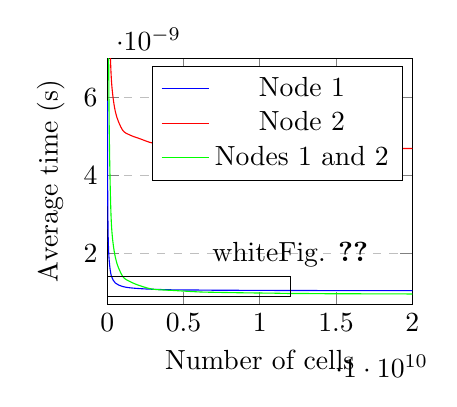
\begin{tikzpicture}
\begin{axis}[
    %title={Average time per cell},
    xlabel={Number of cells},
    ylabel={Average time (s)},
    xmin=0, xmax=20000000000,
    ymin=7e-10, ymax=7e-09,
    legend pos=north east,
    ymajorgrids=true,
    grid style=dashed,
    scaled x ticks={real:10000000000},
    width=0.45\linewidth,
]


\addplot[
    color=blue,
    smooth,
    ]
    coordinates {
    (16777216, 5.9137855257306775e-09)(33554432, 3.600158861705235e-09)(67108864, 2.3944228887557983e-09)(134217728, 1.8066061394555226e-09)(268435456, 1.4282848153795516e-09)(536870912, 1.2414301080363135e-09)(1000000000, 1.152977142857143e-09)(1500000000, 1.119065714285714e-09)(2147483648, 1.0979907321078438e-09)(3000000000, 1.0814785714285714e-09)(4294967296, 1.0668948691870486e-09)(6000000000, 1.0614280952380955e-09)(7000000000, 1.057224693877551e-09)(8589934592, 1.0550598381087185e-09)(10000000000, 1.0521971428571429e-09)(11000000000, 1.0512831168831168e-09)(12000000000, 1.0494261904761902e-09)(13000000000, 1.0495164835164835e-09)(14000000000, 1.0483724489795918e-09)(17179869184, 1.0460199389074528e-09)(25769803776, 1.0433235383104711e-09)(34359738368, 1.042618532665074e-09)(42949672960, 1.0408397897013597e-09)(51539607552, 1.0398679435075748e-09)(60129542144, 1.0400224115927607e-09)(68719476736, 1.0391142235935798e-09)(77309411328, 1.0390710529117357e-09)(85899345920, 1.0391409575406993e-09)(94489280512, 1.0389721250863041e-09)(100000000000, 1.0383371428571429e-09)(103079215104, 1.0382666784737793e-09)(111669149696, 1.038346634051957e-09)(120259084288, 1.0378354666184407e-09)
    };

\addplot[
    color=red,
    smooth,
    ]
    coordinates {
    (16777216, 3.245565720966884e-08)(33554432, 1.8672138452529907e-08)(67108864, 1.1961538876805988e-08)(134217728, 8.379966020584107e-09)(268435456, 6.4965124641145975e-09)(536870912, 5.626971168177468e-09)(1000000000, 5.162437142857143e-09)(1500000000, 5.029282857142857e-09)(2147483648, 4.935963079333305e-09)(3000000000, 4.824004761904761e-09)(4294967296, 4.785867141825813e-09)(6000000000, 4.748461904761905e-09)(7000000000, 4.729608163265305e-09)(8589934592, 4.728251535977636e-09)(10000000000, 4.7160128571428574e-09)(11000000000, 4.704388311688311e-09)(12000000000, 4.696046428571429e-09)(13000000000, 4.699453846153845e-09)(14000000000, 4.695503061224491e-09)(17179869184, 4.688792562644397e-09)(25769803776, 4.678011117946534e-09)(34359738368, 4.6729318065834904e-09)(42949672960, 4.667090252041816e-09)(51539607552, 4.665895609096402e-09)(60129542144, 4.661319378231253e-09)(68719476736, 4.661219593669687e-09)(77309411328, 4.661910694151644e-09)(85899345920, 4.659480016146388e-09)(94489280512, 4.6594083526885355e-09)(100000000000, 4.6598900000000005e-09)(103079215104, 4.659376351074094e-09)(111669149696, 4.6597087530644385e-09)(120259084288, 4.659140748637063e-09)
    };

\addplot[
    color=green,
    smooth,
    ]
    coordinates {
    (16777216, 2.9583752155303957e-08)(33554432, 1.514038017817906e-08)(67108864, 9.290228996958051e-09)(134217728, 5.197258932249886e-09)(268435456, 2.8187840112618036e-09)(536870912, 1.8953390951667517e-09)(1000000000, 1.4202885714285714e-09)(1500000000, 1.277607619047619e-09)(2147483648, 1.1723881055201802e-09)(3000000000, 1.083004761904762e-09)(4294967296, 1.0516730669353688e-09)(6000000000, 1.0138707142857144e-09)(7000000000, 1.003642244897959e-09)(8589934592, 9.929328225553036e-10)(10000000000, 9.85383e-10)(11000000000, 9.808103896103896e-10)(12000000000, 9.733238095238094e-10)(13000000000, 9.729956043956044e-10)(14000000000, 9.68534693877551e-10)(17179869184, 9.647562235061612e-10)(25769803776, 9.547974470825421e-10)(34359738368, 9.519322442689111e-10)(42949672960, 9.487150236964226e-10)(51539607552, 9.463479121526082e-10)(60129542144, 9.423898704045889e-10)(68719476736, 9.409590607642063e-10)(77309411328, 9.429238234010953e-10)(85899345920, 9.43106466106006e-10)(94489280512, 9.422190487384794e-10)(100000000000, 9.425682857142859e-10)(103079215104, 9.416450103301378e-10)(111669149696, 9.416758625225706e-10)(120259084288, 9.41362802167328e-10)
    };

\addplot[
    color=black,
    mark=none,
] coordinates {(0,9e-10) (0,1.4e-09) (12000000000,1.4e-09) (12000000000,9e-10) (0,9e-10)};

\pgfplotsset{
    after end axis/.code={
        \node[above] at (axis cs:12000000000,1.4e-09){\contour{white}{Fig. \ref{result_graph_cell_zoom}}};
    }
}


\legend{Node 1, Node 2, Nodes 1 and 2}
\end{axis}
\end{tikzpicture}
}%
    \subfloat[][Zoomed in]{\label{result_graph_cell_zoom}
\begin{tikzpicture}
\begin{axis}[
    %title={Average time per cell},
    xlabel={Number of cells},
    ylabel={Average time (s)},
    xmin=0, xmax=15000000000,
    ymin=9e-10, ymax=1.4e-09,
    legend pos=north east,
    ymajorgrids=true,
    grid style=dashed,
    scaled x ticks={real:10000000000},
]


\addplot[
    color=blue,
    smooth,mark=diamond,
    ]
    coordinates {
    (16777216, 5.886852741241455e-09)(33554432, 3.59540581703186e-09)(67108864, 2.401748299598694e-09)(134217728, 1.8008887767791747e-09)(268435456, 1.4292880892753601e-09)(536870912, 1.2423399835824965e-09)(1000000000, 1.154624e-09)(2147483648, 1.0980861261487008e-09)(4294967296, 1.067038159817457e-09)(8589934592, 1.0550598381087185e-09)(10000000000, 1.052398e-09)(17179869184, 1.0460199389074528e-09)(25769803776, 1.0433235383104711e-09)(34359738368, 1.042618532665074e-09)(42949672960, 1.0408397897013597e-09)(51539607552, 1.0398679435075748e-09)(60129542144, 1.0400224115927607e-09)(68719476736, 1.0391142235935798e-09)(77309411328, 1.0390710529117357e-09)(85899345920, 1.0391409575406993e-09)(94489280512, 1.0389721250863041e-09)(100000000000, 1.03832e-09)(103079215104, 1.0382666784737793e-09)(111669149696, 1.038346634051957e-09)(120259084288, 1.0377527879817145e-09)
    };

\addplot[
    color=green,
    smooth,mark=square,
    ]
    coordinates {
    (16777216, 2.9002046585083008e-08)(33554432, 1.5357071161270142e-08)(67108864, 9.34590995311737e-09)(134217728, 5.2753239870071416e-09)(268435456, 2.741926163434982e-09)(536870912, 1.903323084115982e-09)(1000000000, 1.4446680000000001e-09)(2147483648, 1.1591557413339615e-09)(4294967296, 1.056760549545288e-09)(8589934592, 9.929328225553036e-10)(10000000000, 9.83829e-10)(17179869184, 9.647562235061612e-10)(25769803776, 9.547974470825421e-10)(34359738368, 9.519322442689111e-10)(42949672960, 9.487150236964226e-10)(51539607552, 9.463479121526082e-10)(60129542144, 9.423898704045889e-10)(68719476736, 9.409590607642063e-10)(77309411328, 9.429238234010953e-10)(85899345920, 9.43106466106006e-10)(94489280512, 9.422190487384794e-10)(100000000000, 9.424657999999999e-10)(103079215104, 9.416450103301378e-10)(111669149696, 9.416758625225706e-10)(120259084288, 9.416818751820496e-10)
    };

\addplot[
    color=indigo,
    smooth,
    ]
    coordinates {
    <generator object <genexpr> at 0x7f11cfe1e410>
    };


\legend{Node 1, Nodes 1 and 2}
\end{axis}
\end{tikzpicture}
}
    \caption{Average time per cell} \label{result_graph_cell_total}
\end{figure*}

\section{Testing the performance} \label{testing}
The implementation has been tested on a cluster of two nodes.
%The test will compare the performance of each single node to the performance of the nodes working together.
%Therefore the exact specifications of the nodes will not be discussed, as the nodes will not be compared nodes to each other.%
Node 1 has an Nvidia GPU with a maximum work-group size of 1024 and Node 2 has an AMD GPU with a maximum work-group size of 256.
That means that the $width$, as discussed in \cref{algorithms}, are 1024 and 256 on Nodes 1 and 2 respectively.
The implementation has been run on the nodes separately and on the nodes as a cluster.
This allows us to compare the time the program needs to return the result.
The values used in figures \ref{result_graph_total} and \ref{result_graph_cell_total} are averages of ten separate runs.
The x-axes represents the product of the lengths of the sequences compared, which is equal to the number of cells in the solution matrix as mentioned in \cref{originalalg}.
The y-axes represents the average time it takes to solve the problem in \cref{result_graph_total} and the average time it takes for one cell to be computed in \cref{result_graph_cell_total}.

\Cref{result_graph_total} shows that the implementation works faster on a cluster than on the individual nodes if the number of cells becomes larger than approximately $0.4 \cdot 10^{10}$ cells.
It also shows that Node 2 takes longer than Node 1 to solve the problem.
This is due to the fact that the width of Node 2 is smaller than the width of Node 1.
If the number of cells is equal to $1.0 \cdot 10^{10}$ Node 1 takes 10.5 seconds to complete, Node 2 takes 47.2 seconds to complete and the cluster takes 9.8 seconds to complete.
The width used in Node 1 is four times as big as the width in Node 2, but the time required to solve the problem is 4.50 times as long.
Therefore we can conclude that Node 2 will be the bottleneck in the cluster.
The implementation does not take into account the difference in performance between nodes, so Node 2 defines the maximum performance of the cluster.

The total width of the cluster is equal to $1024 + 256 = 1280$, and the width of Node 2 is 256.
So Node 2 is going to handle $256 / 1280 = \frac{1}{5}$ of the pillars.
That means that the time the cluster should take is at least one fifth of the time it takes Node 2 to solve the problem.
There is however a small difference between $47.2 / 5.0 = 9.44$ and $9.8$.
This is probably due to the fact that the use of a cluster takes more time to setup and the communication provides some overhead.

The setup taking more time can be seen in \cref{result_graph_cell_total}.
These graphs show the time taken per cell, so extra time taken independent of the number of cells will be visible in these graphs.
The steep decline in time per cell at the left side of the graph is a clear indication that the time to setup is indeed significant.
In these graphs it is also visible that the cluster becomes faster than Node 1 at approximately $0.4 \cdot 10^{10}$ cells, as the amount of time per cell in the cluster drops below the time per cell in Node 1.

From these results we can conclude that optimal number of GPUs in a cluster depend on the size of the sequences compared, when considering the speed of the calculation.
For the specific cluster used in this section $0.4 \cdot 10^{10}$ cells is the size when the cluster is faster than the individual nodes.
The cluster will however never be more efficient than the individual nodes, as the overhead on a cluster persist no matter the size of the cluster.
This means that the user should consider whether or not the superior speed outweighs the inferior efficiency.
\todo{max performance}

\subsection{Comparison of algorithms}
Comparison with the algorithm of De Heus is not useful, since it can not solve the edit distance of sequences longer than the $width$ of a node \cite{Heus}.
The implementation of this paper does not focus on such small sequences, as extra complexity and features results in a significant overhead while computing them.
It is save to say that for comparing small sequences the algorithm of De Heus is more suitable.


\begin{comment}
\subsection{Comparison with CPU implementations}
Comparing the implementation with CPU based algorithms is also not useful, as there is no reliable method to compare the performance of CPUs with GPUs apart from running the implementation on each of them.
The difference between CPUs and GPUs is significantly

A more expensive device will not necessarily have a better performance, so even the cost does not serve as a reliable benchmark.

Even the cost of the devices is not a reliable benchmark as manufacturers do not publish the production cost of a device and use different profit margins.
That is why no such comparison is included.
\end{comment}


\section{Conclusion}
The steps required to distribute the verified implementation of the edit distance are described in \crefrange{q1}{q3}.
The first step is explained in \cref{q1}, which is the division of the algorithm as shown in \cref{division}.
The second step is explained in \cref{q2}, which is the distribution of the pillars among nodes and the communication between the nodes.
Finally, \cref{q3} explains the verification of the new algorithms used in the previous two steps.
The three steps answer the first three subquestions mentioned in \cref{questions}.
Together they answer the research question mentioned in the same section.

The final subquestion is answered in \Cref{testing}, which discusses the performance of the implementation.
%It concludes that the speed of the implementation on a cluster is superior to the speed of the implementation o

\subsection{Future work on the implementation} \label{future}
\Cref{ver:vercors} explains that VerCors offers insufficient support for OpenCL.
A solution would be to improve the tool so that all functionality of OpenCL can be used.
The code of the implementation described in this paper could be used as a simple test.
Once the tool supports OpenCL any ambiguities or inconsistencies can be fixed in the implementation.

There are certain optimisations possible for the MPI algorithm.
As mentioned in \cref{testing}, one node can be the bottleneck of a cluster.
This can be solved by either using the same hardware for every node, or to dynamically divide the work load between nodes.
The dynamic division should allow nodes to negotiate what their tasks will be.

Another optimisation is the use of the CPU parallel to the GPU.
The OpenCL algorithms can be converted to a CPU implementation so that it can help solve the edit distance problem.

The OpenCL algorithms could also be optimised.
The memory used could be limited by using the algorithm of Meyers \cite{Meyers}.
The advantage is that the columns shared between nodes takes less space, so the overhead for sending and receiving the columns should be reduced.
However, a disadvantage is that the algorithm of Meyers requires extra operations per cell and thus reduces the performance of the algorithms.
Therefore, the overall performance of the implementation is not guaranteed to be better than the current implementation.


%\balancecolumns
\bibliographystyle{abbrv}
\bibliography{sigproc}


\end{document}
